\documentclass[10pt,a4paper]{article}
\usepackage[utf8]{inputenc}
\usepackage[english]{babel}
\usepackage{amsmath}
\usepackage{amsfonts}
\usepackage{amssymb}
\usepackage{blindtext}
\usepackage{hyperref} % HYPER LINKS
\hypersetup{ % HYPERREF SETUP
    colorlinks=true,
    linkcolor=blue,
    filecolor=magenta,      
    urlcolor=cyan,
    pdftitle={Overleaf Example},
    pdfpagemode=FullScreen,
    }

\usepackage[left=2cm,right=2cm,top=2cm,bottom=2cm]{geometry}
\usepackage{graphicx} % a package to show images

\usepackage{booktabs}
\usepackage[table,xcdraw]{xcolor}


\title{My first \LaTeX~ document}
\author{SIE doctoral school}
%\date{June 2023}
\date{\today}

\begin{document}
\maketitle % THIS COMMAND WILL CREATE THE TITLE

\section{Introduction}

In this article, we will  deal with basic stuff about \LaTeX.

\tableofcontents



\section{Basic stuff}

You can use \% this way \& with the backslash \textbackslash.
You can create a new \\ line.

\vspace{2cm}

Hello again !

\section{Things about math}

This is dumb text to create a paragraph.
You can write inline math $\alpha = 36$.
\blindtext[1]
It is also possible  to do standalone math this way:

$$
    u(x) = \int_{t=0}^{+\infty} g_{ij}^2(t,x) dt
$$

\noindent With: % Here I don't want to have an indent

\begin{enumerate}
    \item Firstly: $g_{ij} = 5$
    \item And also: $x \in \; ] 0, +\infty [$ % "\;" is a small space 
\end{enumerate}

\noindent You can use numbered equations like this very interresting Eq. \ref{eq:useless}.

\begin{equation}
    z = \sum_{n=0}^N v_n
    \label{eq:useless} % this is the label of the equation.
\end{equation}

\begin{eqnarray}
    a =  5 \nonumber \\ % THIS ONE WILL HAVE NO NUMBER
    b = 12 \\
    0 = 0
\end{eqnarray}

\begin{equation}
    f(x) =
    \left\lbrace
    \begin{split}
        x \mbox{ if : } x > 0 \\
        0 \mbox { otherwise }
    \end{split}
    \right.
\end{equation}

\section{About figures and plots}

\blindtext[1]
We can include graphics inside
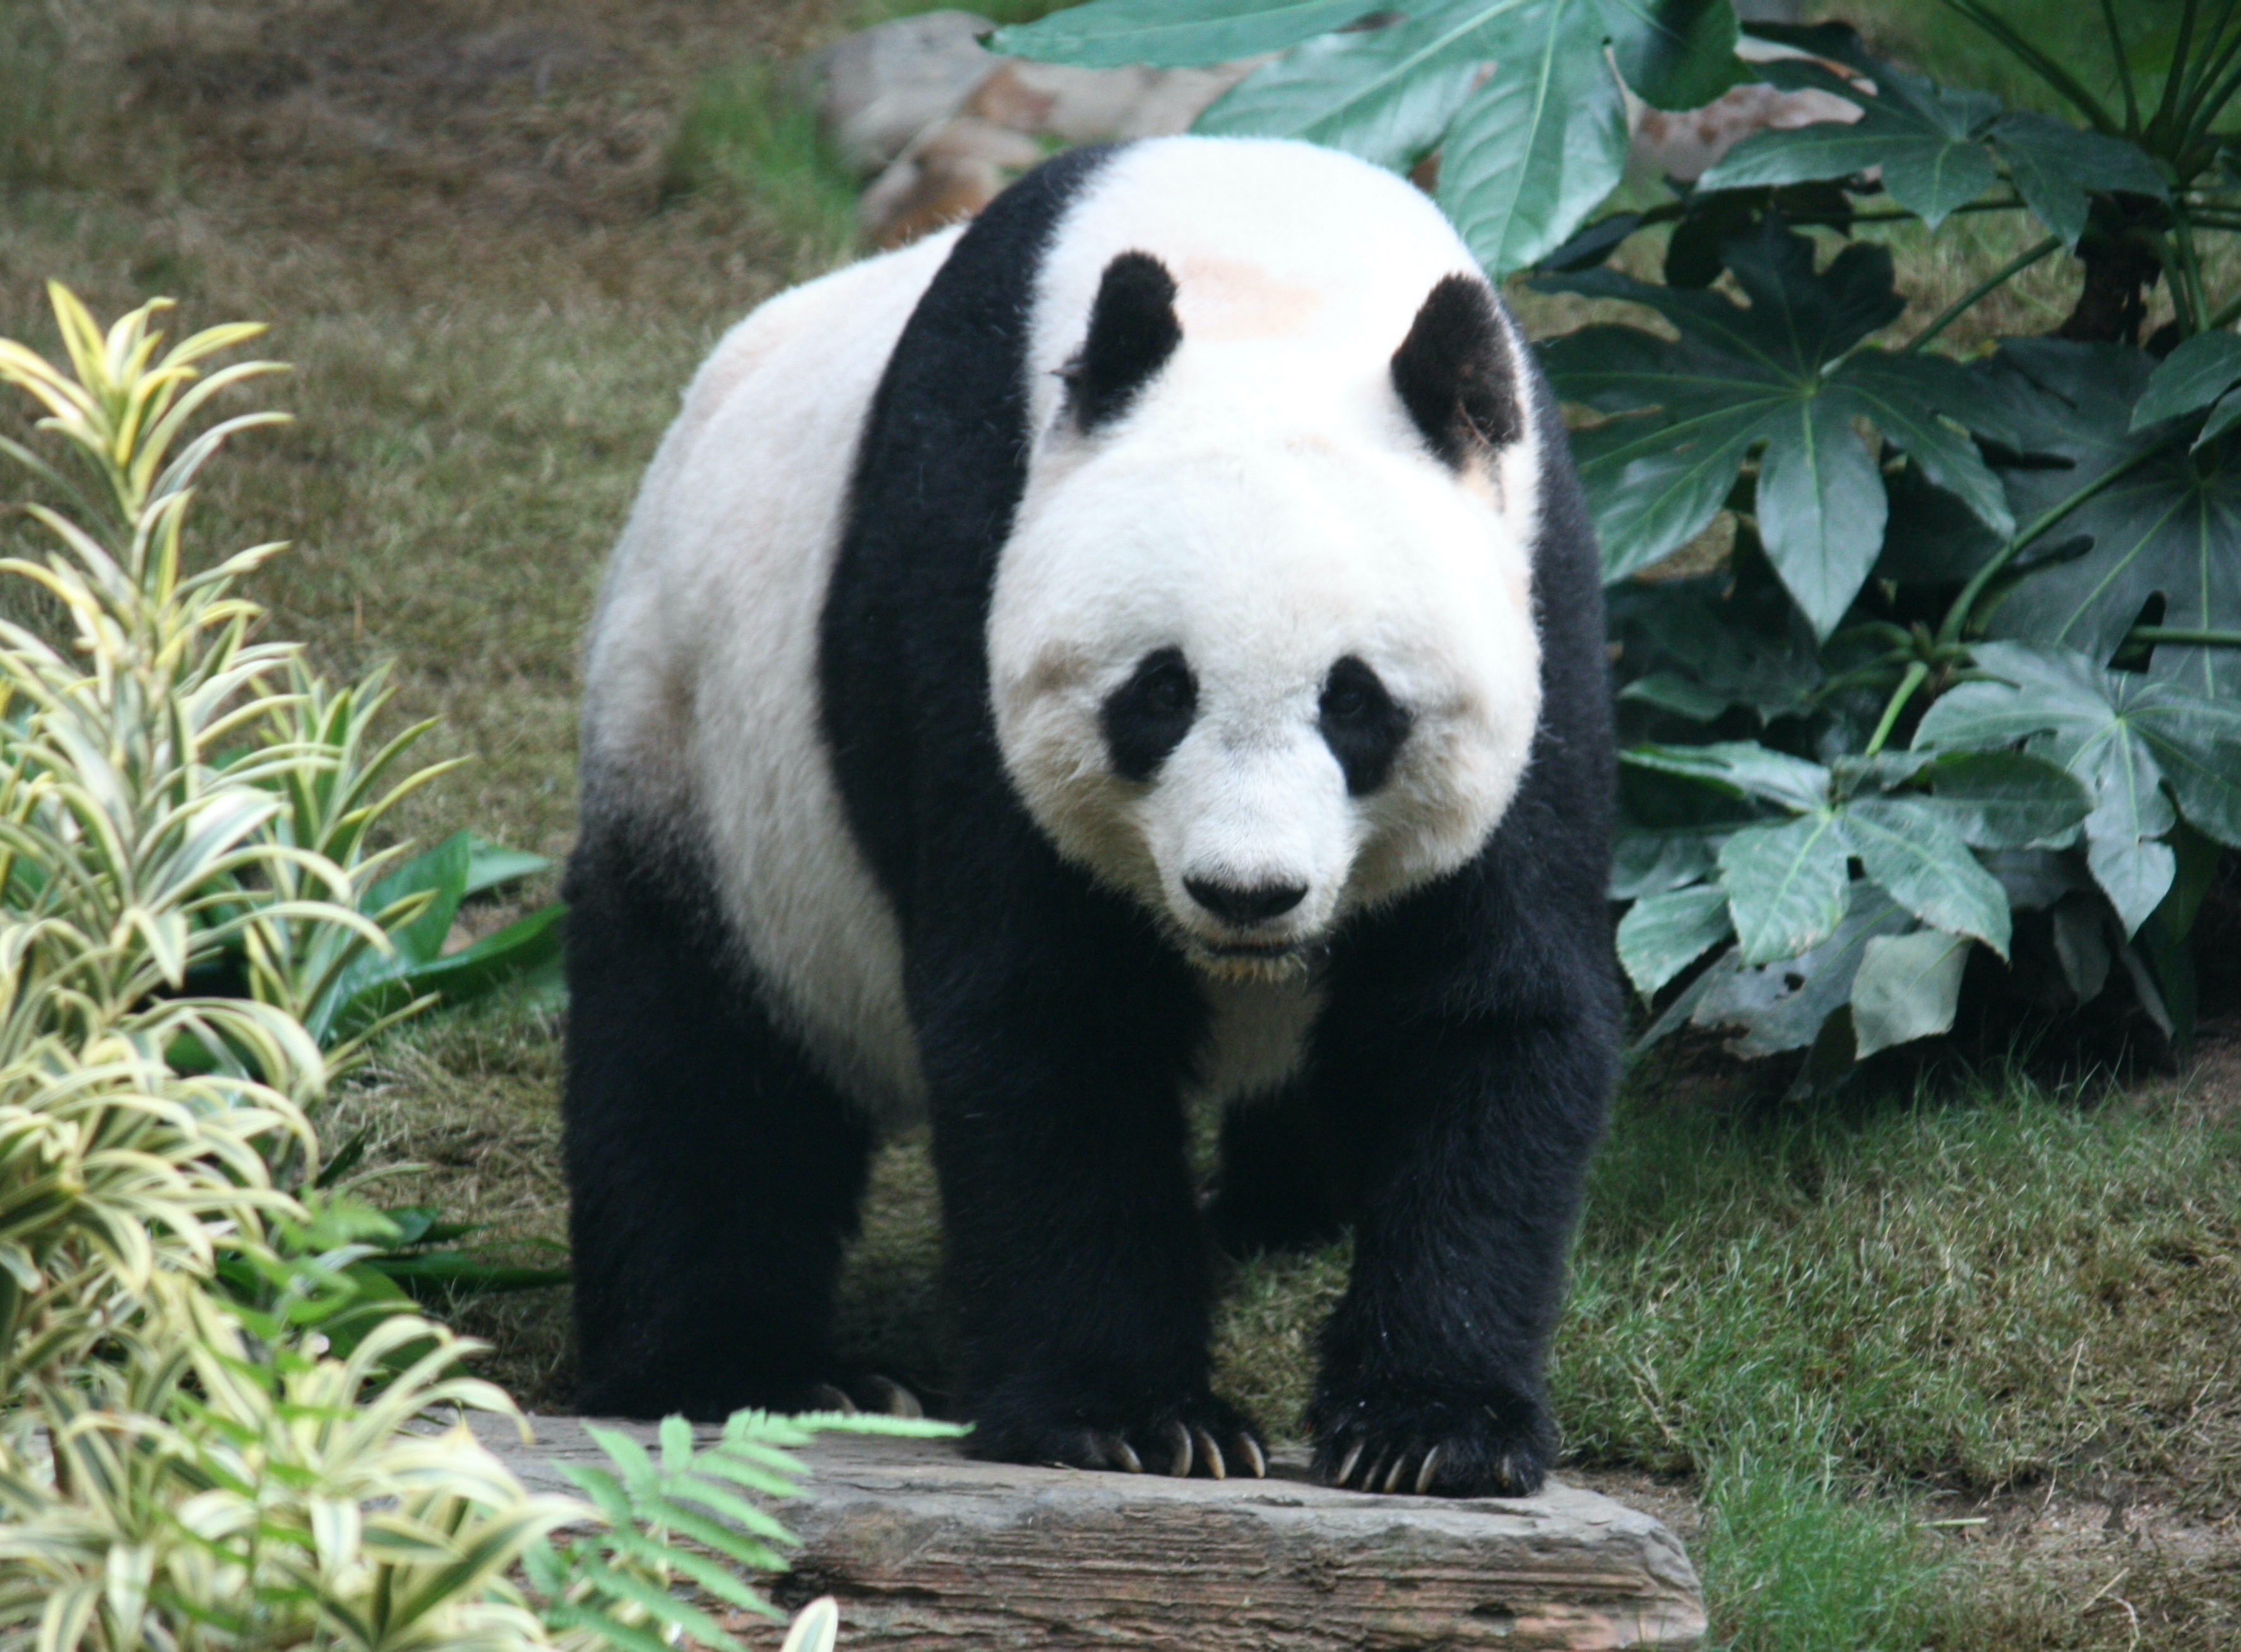
\includegraphics[width = 5mm]{figures/awesome_panda.jpeg}
the text even if it is a bade idea in many cases.
\blindtext[1]
You can see a big panda on Fig. \ref{fig:panda} on page \pageref{fig:panda}.

%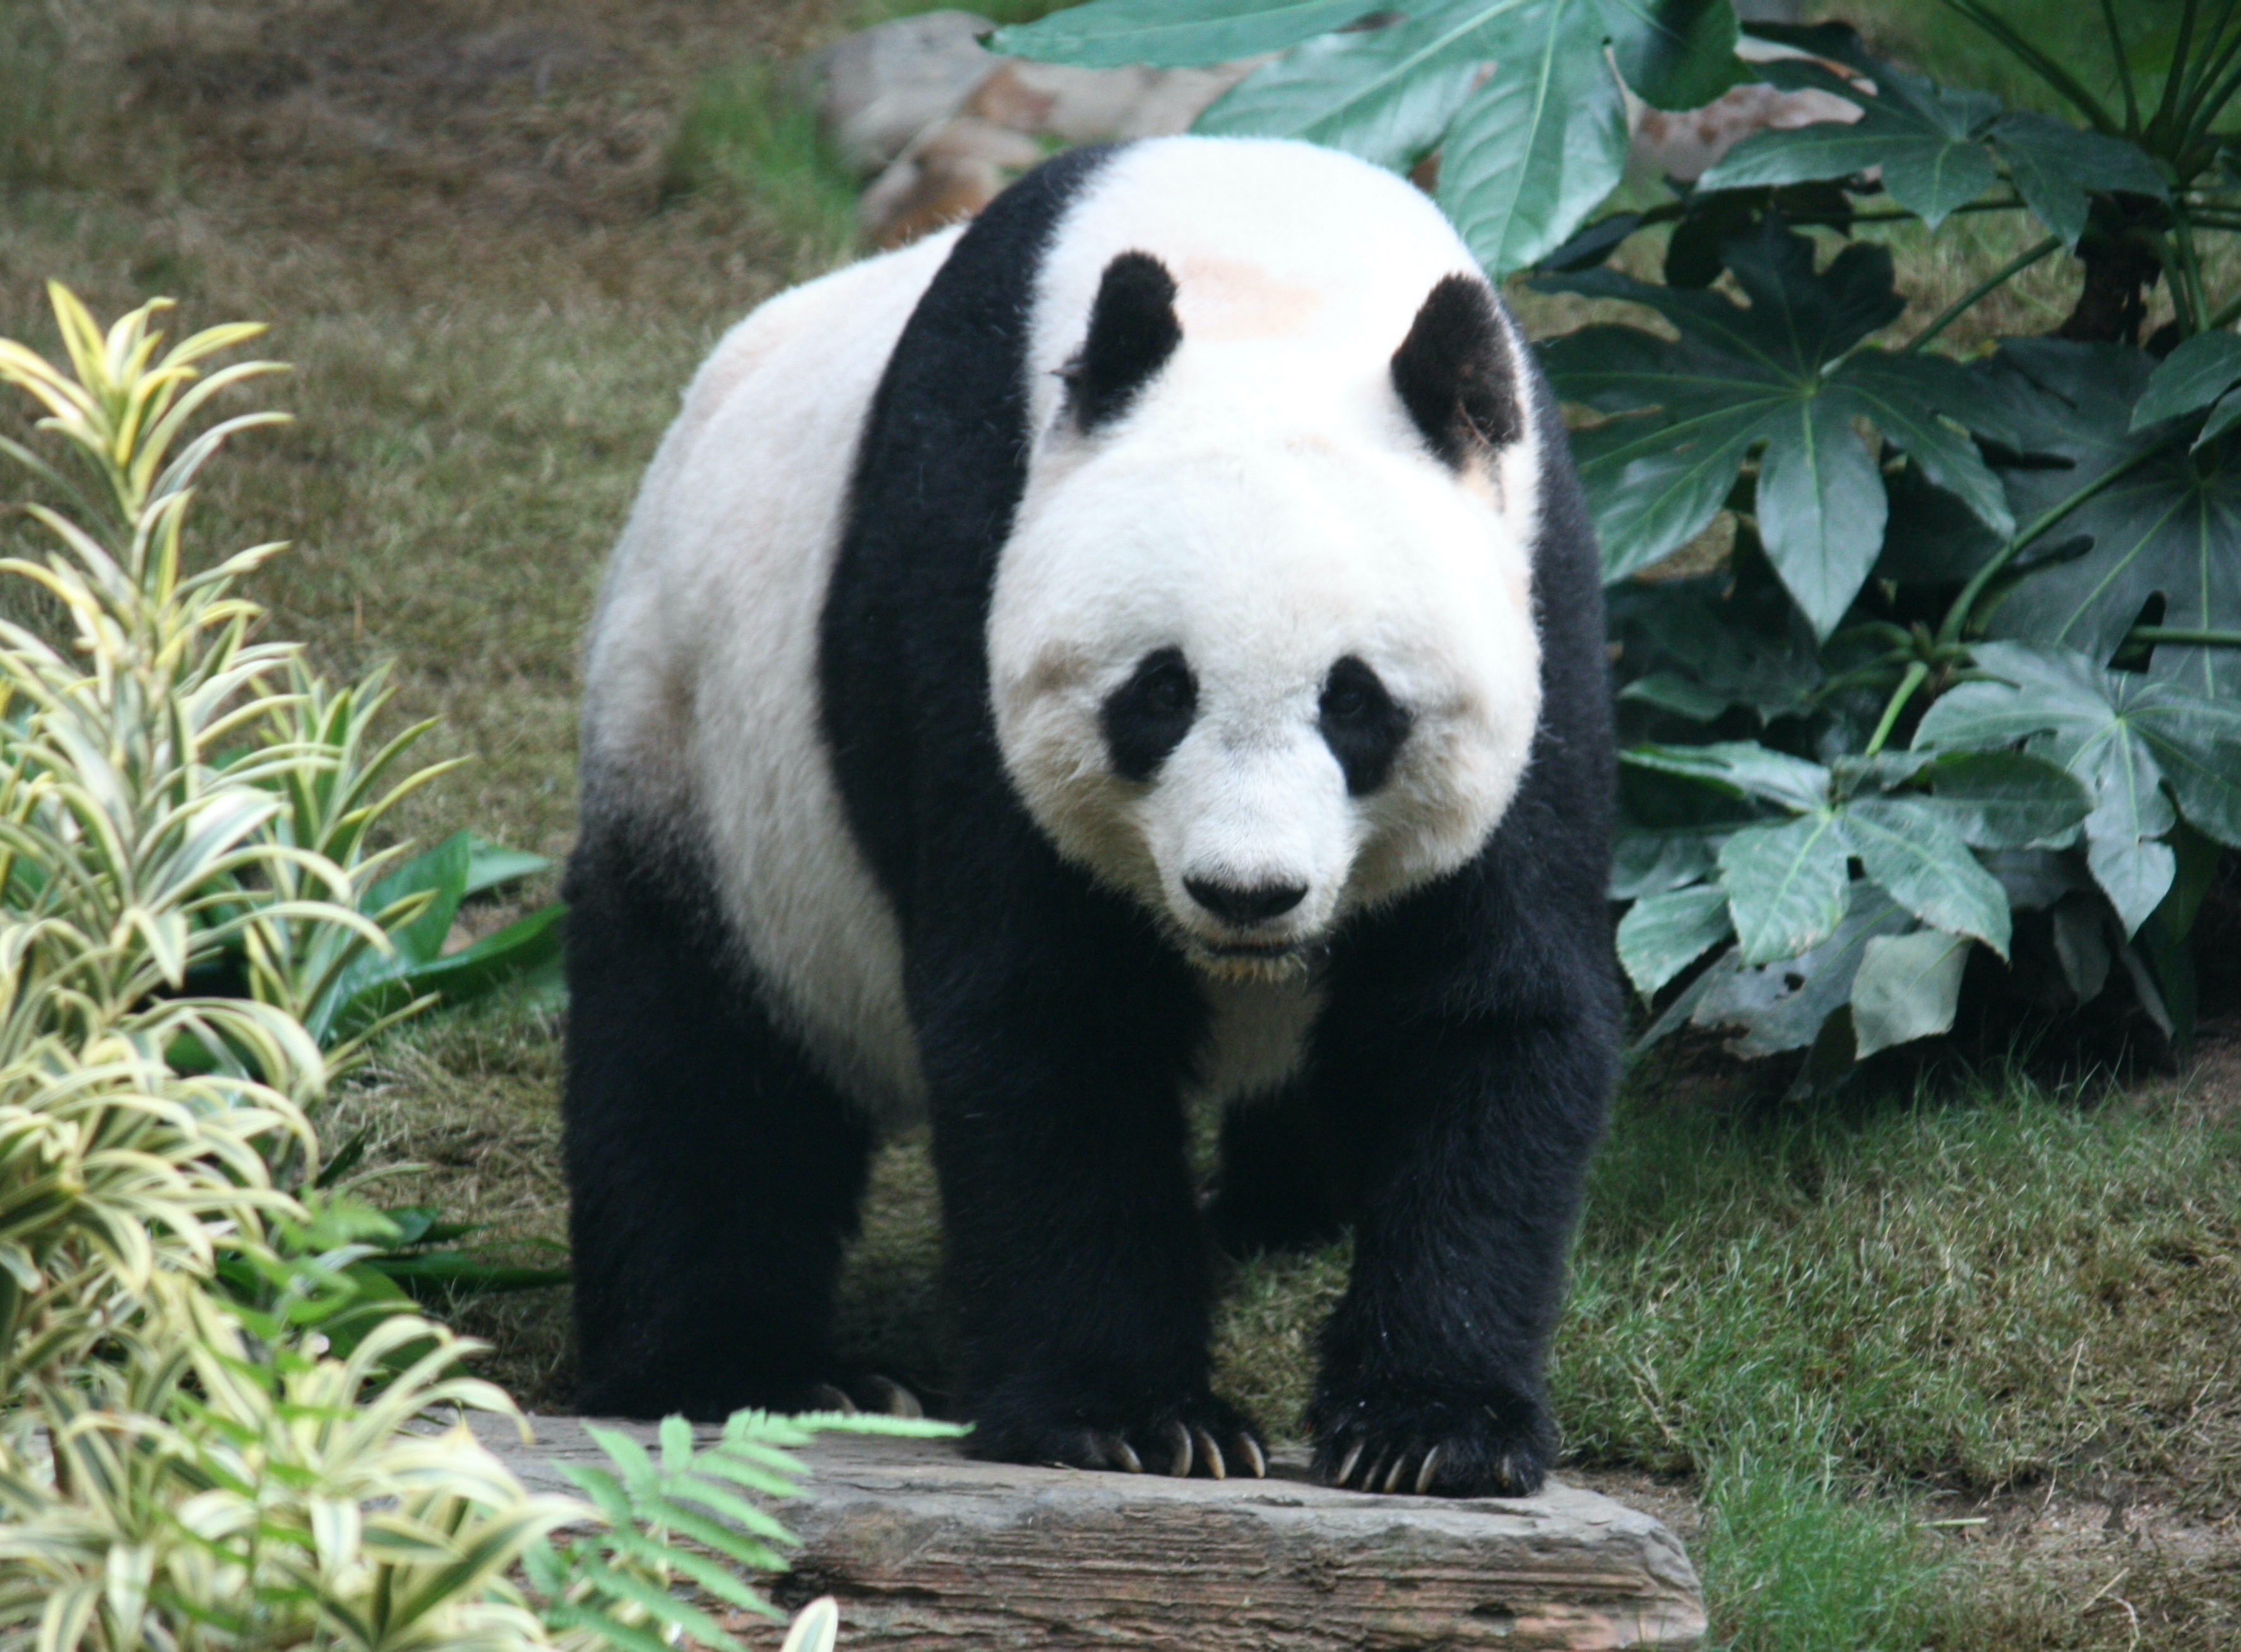
\includegraphics[width = 5cm]{figures/awesome_panda.jpeg}
\begin{figure}
    \begin{center}
        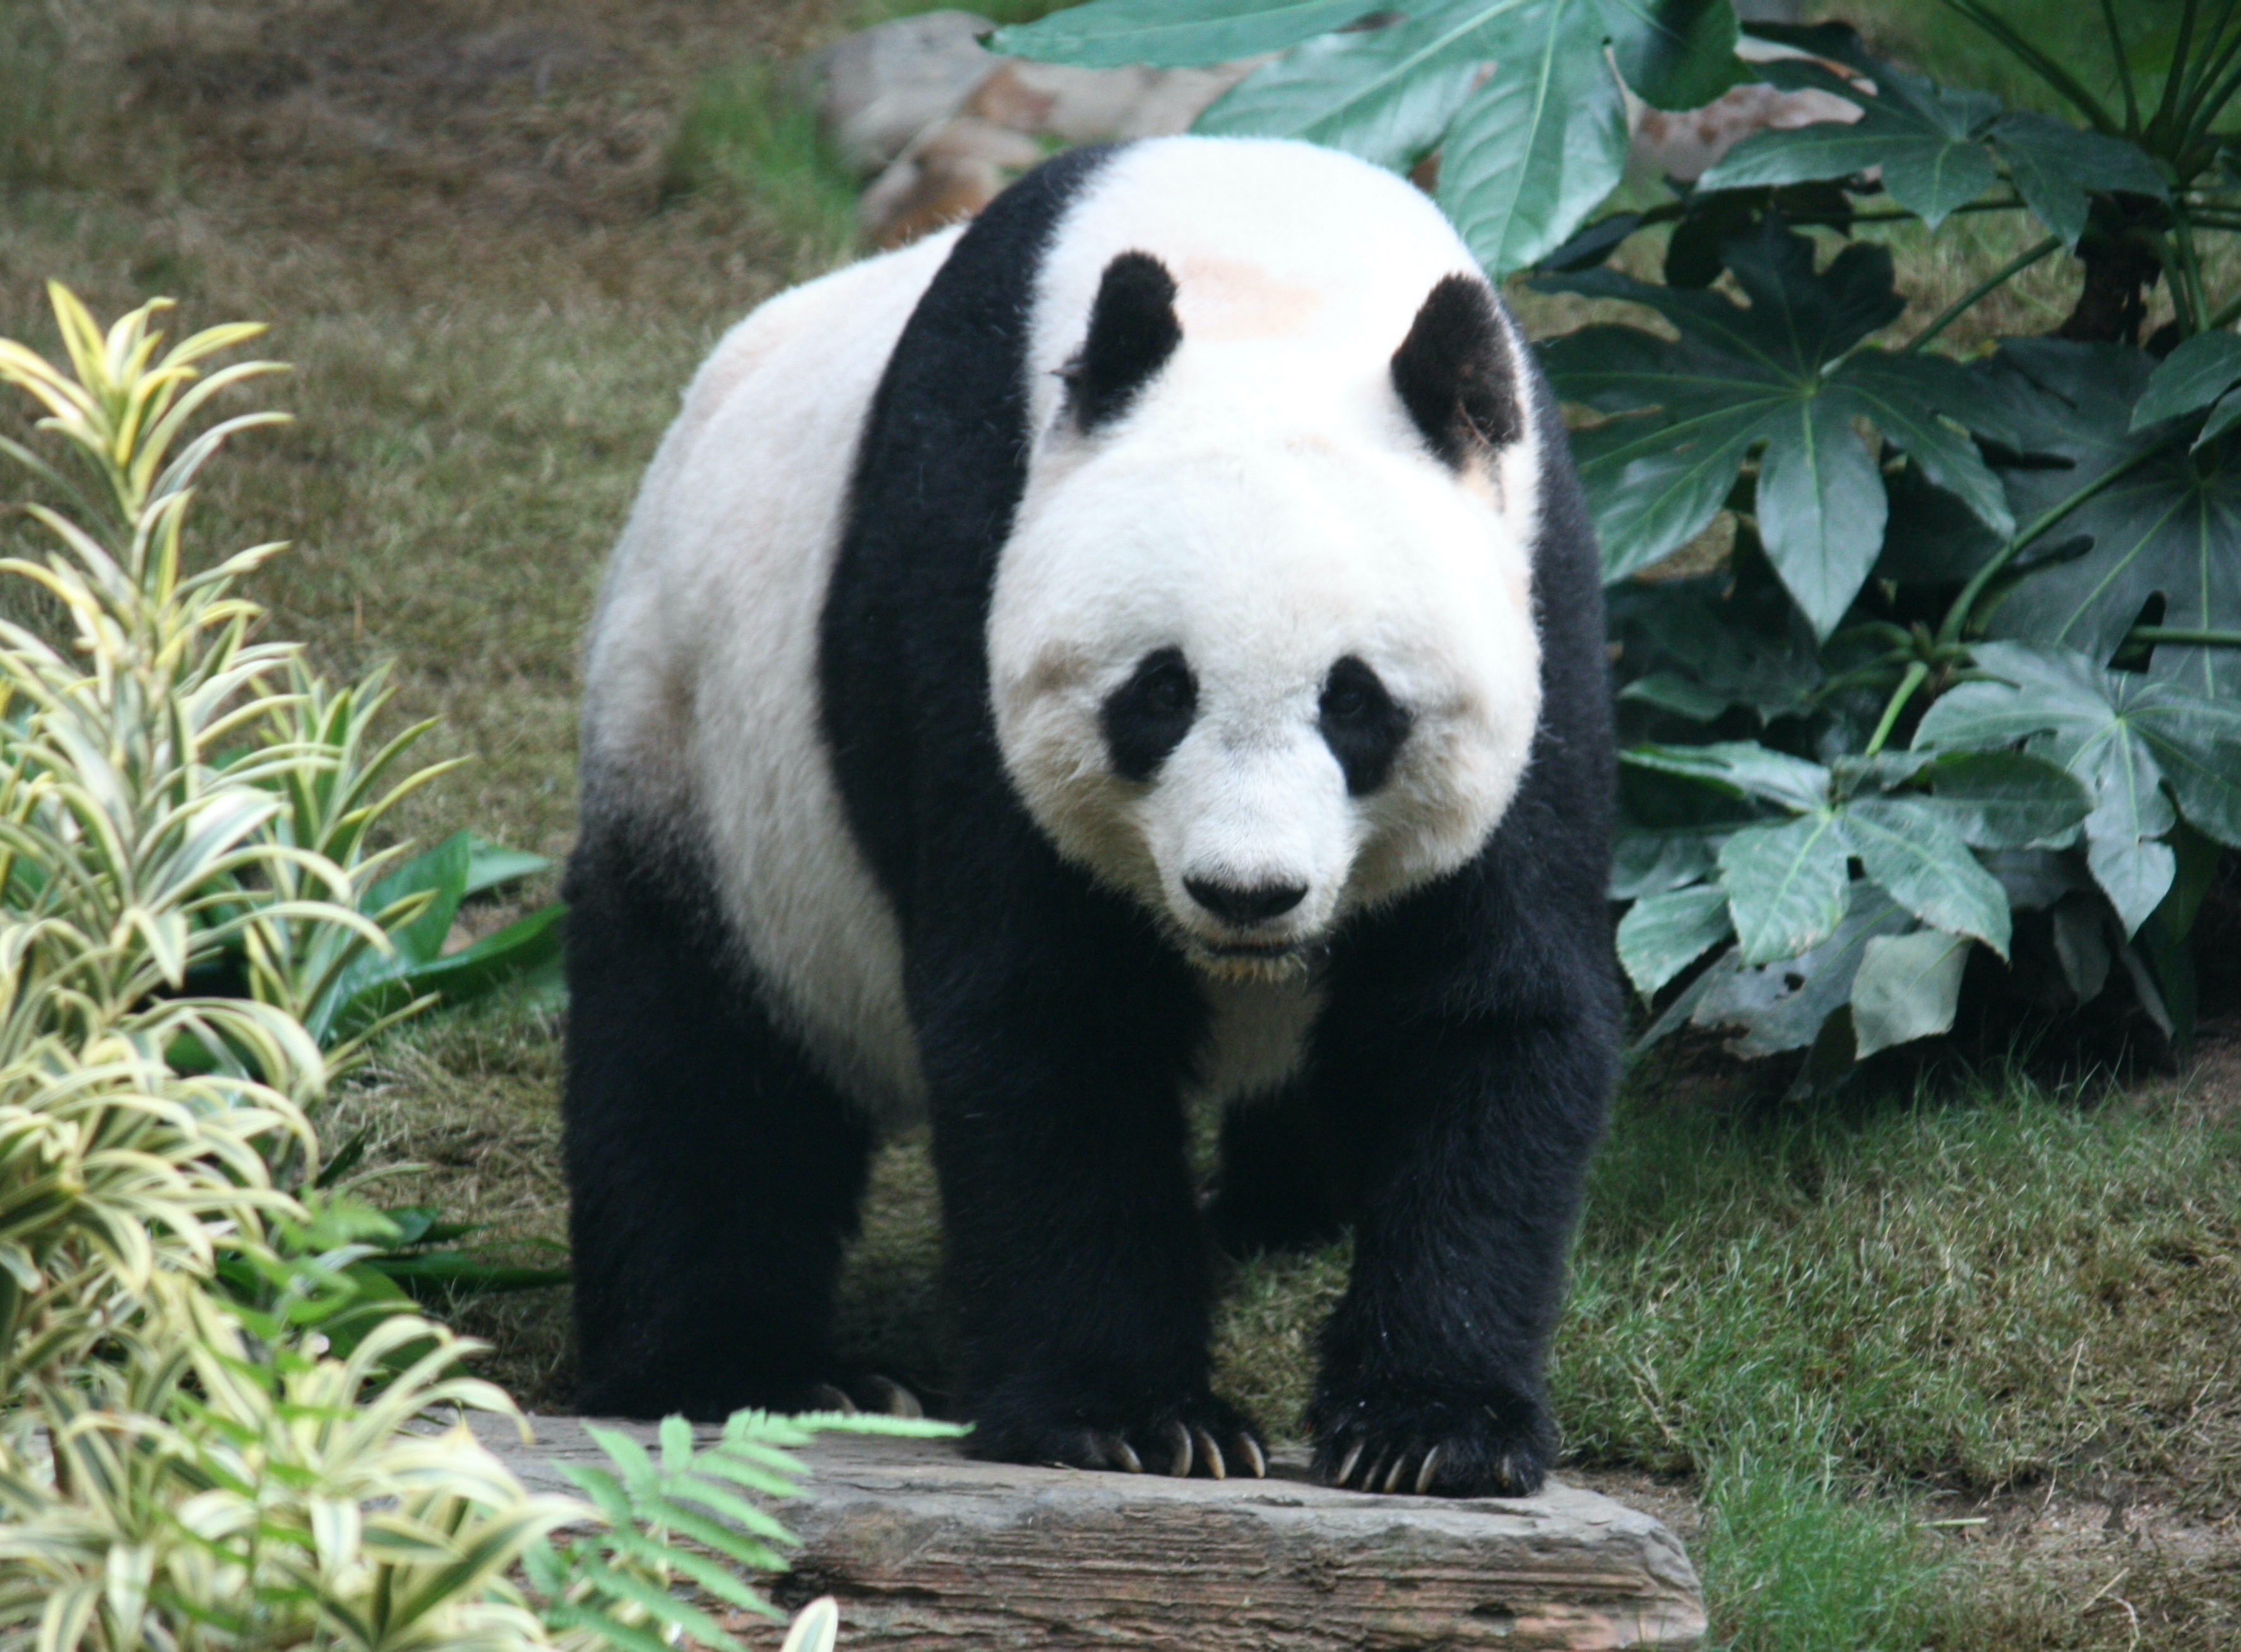
\includegraphics[width = .5\textwidth]{figures/awesome_panda.jpeg}
    \end{center}
    \caption{\blindtext[1]}
    \label{fig:panda}
\end{figure}

\section{Tabulars and tables}

\subsection{Ugly and naive tabular}

\begin{tabular}{|c|c|c|}
\hline 
\textbf{Animal} & \textbf{Size} & \textbf{Weight} \\ 
\hline 
Rabbit & Small & $1$ kg \\ 
\hline 
\end{tabular} 

\subsection{Prettier tables with booktabs}

%\usepackage{booktabs} % DON'T FORGET TO ADD THIS ON TOP

\begin{tabular}{ccc}
\toprule
\textbf{Animal} & \textbf{Size} & \textbf{Weight} \\ 
\midrule
Rabbit & Small & $1$ kg \\ 
Rabbit & Small & $1$ kg \\ 
Rabbit & Small & $1$ kg \\ 
Rabbit & Small & $1$ kg \\ 
\bottomrule
\end{tabular}

\subsection{Using Tablesgenerator}

Using \url{www.tablesgenerator.com}.

% Please add the following required packages to your document preamble:
% \usepackage{booktabs}
% \usepackage[table,xcdraw]{xcolor}
% If you use beamer only pass "xcolor=table" option, i.e. \documentclass[xcolor=table]{beamer}
%\begin{table}[]
\begin{tabular}{@{}ccc@{}}
\toprule
\cellcolor[HTML]{6665CD}Name                    & \cellcolor[HTML]{6665CD}Here & There                      \\ \midrule
\rowcolor[HTML]{6665CD} 
\multicolumn{1}{|c|}{\cellcolor[HTML]{6665CD}1} & \multicolumn{2}{c|}{\cellcolor[HTML]{6665CD}08:15}        \\ \midrule
\multicolumn{1}{|c|}{2}                         & \multicolumn{1}{c|}{13:30}   & \multicolumn{1}{c|}{17:30} \\ \midrule
\multicolumn{1}{l}{2bis}                        & \multicolumn{1}{l}{14:30}    & \multicolumn{1}{l}{18:30}  \\ \bottomrule
\end{tabular}
%\end{table}

\subsection{Table environment}

The table environment make table floating objects and allows you to add a caption and a label to your tabular.
\blindtext[3]
I want my table to be here.

\begin{table}[htb] % A FLOATING ENVIRONMENT FOR TABLES
\begin{center}
\begin{tabular}{ccc}
\toprule
\textbf{Animal} & \textbf{Size} & \textbf{Weight} \\ 
\midrule
Rabbit & Small & $1$ kg \\ 
Rabbit & Small & $1$ kg \\ 
Rabbit & Small & $1$ kg \\ 
Rabbit & Small & $1$ kg \\ 
\bottomrule
\end{tabular}
\end{center}
\caption{A table with a legend.}
\label{tab:useless_table}
\end{table}


\blindtext[3]

\section{About bibliography}

To use bibliography, you need to create a Bibtex file. 
For example, I can cite \cite{hawking2010nature} and \cite{stromberg2014get}.

\bibliography{biblio} % RELATIVE PATH TO THE BIB FILE
\bibliographystyle{plain}



\end{document}